%!TEX root = ../document.tex
\chapter{Theoretical perspective and concepts for analysis}

In this chapter we will lay forth the theoretical perspective and theoretical concepts we will apply in this thesis. First we will introduce the \emph{sociocultural perspective} and highlight some key points including \emph{institutional practices}, \emph{zone of proximal development} and \emph{scaffolding}. Further we will look at \emph{multiple external representations} and lastly the concept and method of \emph{Inquiry learning}.

\section{Sociocultural perspective}

%The sociocultural perspective may be thought of as the synthesis of the behavioristic thesis and cognitive antithesis. The behavioristic model focuses on the role of the individual and the notion that knowledge arises through individual drill and practice. In contrast, the cognitive model focuses on the environment and the notion that the environment provides raw material for testing innately conceived hypotheses, thus focusing on instruction methods and acquisitional models. The sociocultural perspective considers the individual in the context of their environment, with a focus on means of mediation between the two. Thus, action is the primary unit in sociocultural analysis, which will be elaborated further in the following paragraphs. 

%The sociocultural perspective considers the individual in the context of their environment, with a focus on means of mediation between the two. Thus, action is the primary unit in sociocultural analysis, which will be elaborated further in the following paragraphs. 


In a biological sense the human species has not evolved significantly the last ten thousand years or so. In fact, changes in our gene pool are only minor, and can’t explain the difference between modern people and people of the Stone Age. Still we are able to achieve tasks that would have been impossible for our ancestors \citep{saljo2001laering}.

The explanation of this discrepancy from a sociocultural perspective becomes evident when one takes into account the \emph{tools} and \emph{signs} we use to mediate the world. We have created a culture where each of the \emph{tools} and \emph{signs} we use has a long history embedded in them. For instance if you are given the multiplication problem 122\texttimes284, you can flip up a calculator and get the answer instantaneously. Similarly, if you were to solve the multiplication problem 7\texttimes4 you can look up in a multiplication table and find the answer easily. These \emph{cultural tools} (calculator and multiplication table) enable you to make sense of the world in a different way than our ancestors. 

From the example given above we can see that there is an “irreducible tension” between the agent and the cultural tool \citep{wertsch1998mind}. Without the multiplication table you would not be able to solve the problem. But the multiplication table is not enough, as it would have been useless without a skilled user. The goal of a sociocultural approach is therefore to: 

\begin{quote}
Create an account of human mental processes that recognizes the essential relationship between these processes and their cultural, historical, and institutional setting.\citep{wertsch1998mind} 
\end{quote}

This means that the unit of analysis is human action, and how it is mediated by cultural tools, or “agent-acting-with-mediational-means” \citep[\citealp{wertsch1993sociocultural} cited in][]{wertsch1998mind}. The mediated action can never be understood by the properties of only the agent, the mediational means, or the cultural, historical and institutional setting of the mediated activity. An example of this is $\text{H}_2\text{O}$: one can not understand what makes up water if one analyses hydrogen and oxygen separately. The characteristic of the whole is not made up by the characteristics of the elements \citep{vygotskiui1978mind}. Another example is the track-and-field event of pole vaulting. 
\begin{quote}
The pole by itself does not magically propel vaulters over a cross bar; it must be used skillfully by the agent. At the same time, an agent without a pole or with an inappropriate pole is incapable of participating in the event \citep{wertsch1998mind}. 
\end{quote}
So while analysis of the elements in isolation may be informative, we will never understand the big picture without taking into account the relation between the mediational means, the agent, and the sociocultural context. 

\subsection{Tools and signs}
One important distinction to make when talking about mediated activity is that of tools (physical tools) and signs (psychological tools) \citep{vygotskiui1978mind}. While they are similar in that they can play a mediating role in activity, they are different in the ways they orient human behavior. The tool is externally oriented and must lead to change in physical objects. A basic example of a tool is a hammer. An agent can mediate her activity toward the external world by using the tool to crush a coconut. A sign on the other hand is internally oriented and “changes nothing in the object of psychological operation” \citep{vygotskiui1978mind}. Examples of signs are: diagrams, drawings, language, or as mentioned above, multiplication tables. “It is a means of internal activity aimed at mastering oneself” \citep{vygotskiui1978mind}. 

Another illuminating example of the difference between tools and signs is that of a child presented with a birthday cake. The child does not immediately start eating, but waits until “happy birthday” has been sung and she has blown out the candles. In that sense the cake is a sign as it represents a lot more than just food in the mind of the child. It signifies that she is a year older, that she is going to get presents afterwards, that she is celebrated, etc. On the other hand, from the parents’ point of view, the cake can be used to signify that she is a year older and has new responsibilities in the society. 

If we look at the same example from a behavioristic point of view, another situation emerge. The behavioristic model focuses on the role of the individual and the notion that knowledge arises through individual drill and practice. The girl would therefore know from previous experience that cake tastes good, and immediately start to dig in. 

\emph{In contrast}, the cognitive model focuses on thought processes and the notion that the environment provides raw material for testing innately conceived hypotheses. The reason for the girl not eating the cake would therefore be an internal thought process and the context in which the cake is placed would play a minor role. 

\subsection{Implications for learning}
“From a sociocultural perspective learning is understood as mastery and appropriation of cultural tools” \citetext{Wertsch, 1998, Säljö, 1999, 2001, cited in \citealp{mifsud2010reconsidering}}. \citet{wertsch1998mind} does however make a distinction between knowing how to use a cultural tool (mastery) and making a cultural tool one’s own (appropriation). Appropriation can be to take the mastery one step further. Oxford dictionary defines it as “the action of taking something for one’s own use”, or as \citet{wertsch1998mind} puts it “making a cultural tool one’s own”. One example of this is a person who has mastered the cultural tool "chords" on a guitar and later appropriates them to a song. It should however be recognized that both mastery and appropriation does not always happen. For example, a person could master the chords on the guitar and perform them flawlessly in class, but dismiss them as terribly ugly at home. Likewise, a person can appropriate chords to a song without mastering the chords themselves.

When we then ask what learning is from a sociocultural perspective, we are also asking “‘which cultural tools are valued?’, and ‘In which contexts do they apply’” \citep{mifsud2010reconsidering}. In order to give an answer to these questions, we have to take into account the cultural, historical and institutional context of the mediated activity. 

To set the scope for our thesis we have decided to place an emphasis on the institutional part of the context, while still acknowledging that the context has cultural and historical aspects.  

\subsection{Social practices}
With a sociocultural perspective on learning, we see external and internal processes as intertwined. By this we try to see student interactions with artefacts and each other as embedded in a cultural, historical and institutional practice, meaning that we take into account the relation between the mediational means, the agent and her contexts. These practices can be embedded into cultural artefacts or as \citet{furberg2009socio} states: "computer based environments can embed such practices in the design". She mentions two types of social practices embedded in Web-based inquiry learning environments: \emph{scientific inquiry} and \emph{institutional practices}.  Scientific inquiry is often expressed by encouraging students to do ideal scientific activities e.g., hypothesis generation, evaluating evidence and constructing explanations. Institutional practices can be expressed in terms of school science as an institutional practice, for example by means of tools that enable the teacher to supervise the students, assignments that makes the students think as if they are beeing assessed, or tools for the students to test their own skills. These practices can also include metaphores taken directly from the institution of school, for example as shown in figure~\ref{fig:scrshotviten} where all the assignments states that you need to be logged in as a student to type in an answer. These "embedded institutional practices can be, and often are, at odds with the ideal practices of scientific inquiry." \citetext{\citealp{chinn2002epistemologically}, referenced in \citealp{furberg2009socio}}

\begin{figure}
\centering
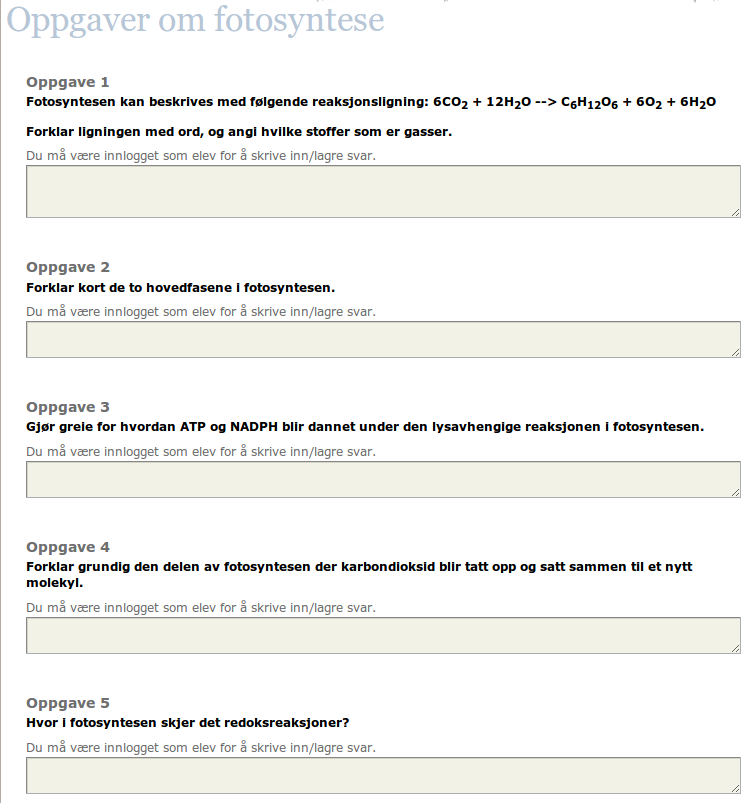
\includegraphics[width=1\textwidth]{img/theoretical/vitenassessment.png}
\caption{Screenshot from viten.no showing student-role metaphor}
\label{fig:scrshotviten}
\end{figure}

Likewise \citet{jimenez2000doing} pose that "doing science" has an obstacle named "doing school". Where "doing science" refers to argumentation or dialog characterized by “construction, representation, evaluation of knowledge claims and investigative methods” \citep{jimenez2000doing}. While "doing school" refers to what actions and activities students and teachers do that instantiates rituals, routines and expectations in educational settings, e.g., review homework assignments, take lecture notes, take tests, complete lab activities etc. These school activities are often taken for granted by researchers, and serve as obstacles for "doing science", which tend to be a focus-area for researchers. Such research have contributed to the understanding of students argumentation and knowledge claims, but as \citet*{furberg2008students} suggests; a more holistic view is needed to get a rich understanding of the complexity of students' meaning making. Meaning that both the dimension of "doing school" and the dimension of "doing science" needs to be taken into account. 

\subsection{Spontaneous and scientific concepts} \label{cha:spontaneous_scientific}
In the early stages of life, children learn for the most part by experience. Skills such as mastering the native language, walking, running are learned through trial and error. This means that the knowledge of a concept is linked to the concrete experience where she was presented with the concept. A child who is presented with the concept of "brother" by a pointing gesture toward her brother, will at first only associate the word "brother" with that specific person. This is what \citeauthor{vygotsky2012thought} calls \emph{spontaneous concepts}

An only child on the other hand, will be introduced to the concept of brother through other concepts. A parent can for instance say that "brothers are boys who have the same parents". The concept of brother will then be a general concept for the child, not linked to any concrete experiences, but to the concepts of "boys" and "parents". This is what \citeauthor{vygotsky2012thought} calls \emph{scientific concepts}

The major difference between these two types of concepts is that spontaneous concepts are developed outside the conceptual framework and only linked to concrete experiences in the mind of the learner. If we presented the child having a brother with the abstract problem of a "brother's brother" \citep{vygotsky2012thought} he would become confused, as his only knowledge of the concept of brother is with situations with his brother

In contrast, scientific concepts are developed within a conceptual framework. They are immediately given a place within the system of concepts, i.e., explained by their relation to other concepts. As a result, the child is consciously aware and able to reflect on the concept \citep{van1998concept}. If we presented the only child with the abstract problem of a "brother's brother", he would most likely be able to solve it because of the concepts relation to other concepts in the mind of the child. 

Another example is how children develop a concept of time. In the early stages of life, a child may think that day and night is analogous to light and darkness. This is the spontaneous concept saturated by experience. It is only later in school he learns the scientific concepts of the earth's rotation and its relation to the sun and the moon, which marks days and years. This information has not been appropriated by experience, as the child has not been to space and experienced it, the information is constructed using different signs linked together by the instructor. 

\begin{figure}
\centering
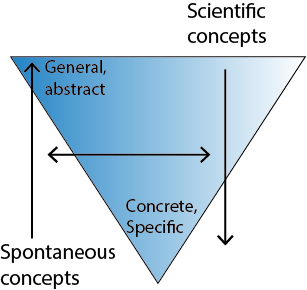
\includegraphics[width=0.6\textwidth]{img/theoretical/conceptpyramid.png}
\caption{The concept pyramid}
\label{fig:conceptpyramid}
\end{figure}

The relationship between these two categories can be explained as an upside-down pyramid. On the top we have the scientific concepts, which are general and abstract. And on the bottom we have the spontaneous concepts, which are specific and concrete. The concepts then move toward each other. The scientific concepts move downwards "toward greater concreteness" in a deductive manner, whereas the spontaneous concepts move "upward toward greater abstractness" \citep{vygotsky2012thought} in a inductive manner.

Even though the concepts move in opposite directions, there is a mutual dependency between them. In Vygotski{\u\i}'s terms: "In working its slow way upwards, an everyday concept clears a path for a scientific concept and its downward development". This means that "the development of a spontaneous concept must have reached a certain level for the child to be able to absorb a related scientific concept" \citep{vygotsky2012thought}. It is therefore essential for the teacher to bring the spontaneous concepts up to a level that makes the scientific concept within reach for the student. By doing this, the student will have the experience, and the related concepts necessary for constructing knowledge of an abstract concept. 

This brings us further to the zone of proximal development, as students who lack consciousness and control over the spontaneous concepts can "find this control within the zone of proximal development" \citep{vygotsky2012thought}.

\subsection{Zone of proximal development}
Lev Vygotski{\u\i}, was concerned with the relationship between learning and development, and argues that the theorists of his time such as Piaget, James and Koffka does not provide an adequate view of this. He finds that learning and development are interrelated, and that this relationship has some specific applications in school-learning. \citep[p. 84]{vygotskiui1978mind} Thus, in order to describe these issues he introduces the concept Zone of Proximal Development (ZPD), and defines it as follows:

\begin{quote}The distance between the actual developmental level as determined by independent problem solving and the level of potential development as determined through problem solving under adult guidance or in collaboration with more capable peers \citep[p. 86]{vygotskiui1978mind}
\end{quote}

\begin{figure}
\centering
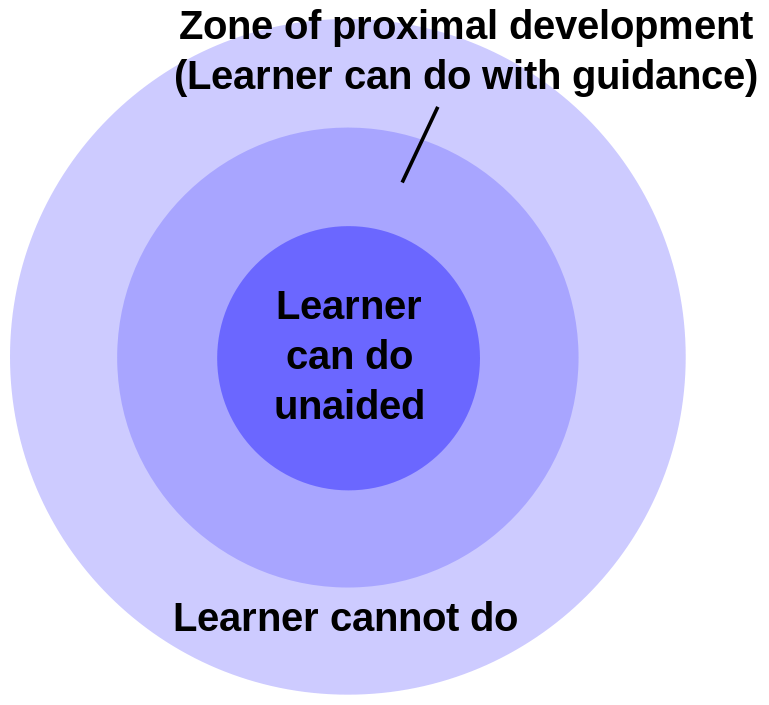
\includegraphics[width=0.5\textwidth]{img/theoretical/zpd.png}
\caption{The zone of proximal development}
\label{fig:zpd}
\end{figure}

The actual developmental level is in other words determined by looking at what a person can do alone. Vygotski{\u\i} found that this traditional way of determining a person's mental development did not hold in school learning, as it only describes what functions in a person that have already been matured. He therefore introduces a new developmental level, the potential development, which can describe the functions in a person that are in the process of maturation. The actual development of a person is therefore the end product of developing, while the potential development is the state and process of developing. The ZPD can be used as a tool by teachers and instructors to delineate the immediate future of their students, i.e., their actual development of tomorrow.

Vygotski{\u\i} proposes further that ZPD is an essential feature of learning, which distinguishes learning from development, but at the same time provokes developmental processes that would not be possible without learning. In other words,

\begin{quote}It awakens a variety of internal developmental processes that are able to operate only when the child is interacting with people  in  his  environment  and  in  cooperation  with his peers. \citep[p. 90]{vygotskiui1978mind}
\end{quote}

By applying the ZPD to learning-situations, the key takeaway is that the analysis alters the traditional view of knowledge or mastery, and shows that the constructed knowledge provides the basis for further development. A great example of this is the process of mastering native language, which initially is learned as a means of communication between the child and other people. The use of language first happens on a social level, in the interaction with people, and is later developed to internal speech and becomes a means to organize thought, i.e., an internal mental function . Vygotski{\u\i} calls this concept the \textit{duality of learning} \citep{vygotskiui1978mind}. 

Another classic example is that of a child trying to grasp a ball. At first the gesture means nothing to the child, but when the mother realizes that the gesture indicates something, the situation changes dramatically. When she gives him the ball, as a result of the hand gesture, the "grasping movement changes to the act of pointing" \citep{vygotskiui1978mind}. This means that the operation that was initially an external activity is now "reconstructed and begins to occur internally" \citep{vygotskiui1978mind}. Thus, \textit{externalization} precedes \textit{internalization}. 

With this in mind, a teacher can understand what developmental processes is maturing in their students, and from that give adapted challenges, show partial solutions and in general tailor what to say and teach next. From this perspective, development is lagging behind learning, and the challenge for the teacher becomes to teach ahead of development, but at the same time not too far ahead. This leads us to the concept of scaffolding, which can be argued to be a refinement of ZPD. 

\subsection{Scaffolding}
Vygotski{\u\i}'s Zone of Proximal Development is the distance between what a person can do alone and what he can do with help from a More Knowledgeable Other (MKO). What types of help and how the MKO should provide it, has not been a focal point for Vygotski{\u\i}. Although \citeauthor*{wood1976role} does not reference to any Vygotski{\u\i}an literature, the term scaffolding introduced by them in 1976, bears resemblance to the very idea of ZPD. As they put it:

\begin{quote}Scaffolding consist essentially of the adult "controlling" those elements of the task that are initially beyond the learner’s capacity, thus permitting him to concentrate upon and complete only those elements that are within his range of competence \citep{wood1976role}
\end{quote}

Thus, scaffolding can be applied by MKOs in order to keep the learning process within the learner’s ZPD. There is a is a nuanced balance for how much guiding is needed and a key point is that a person's ZPD is personal, thus a scaffold should be personally adjusted. An example can be if we were to teach two persons how to take a picture with a professional DSLR camera, one being an old woman (Mary) with little insight in technology, the other a young man (Ryan) who has grown up with technology. It is obvious that the two persons have different cultural backgrounds and taking a picture have different meanings to them, hence the tutoring of them need to be differently tailored. In the following section we will go through the six steps of scaffolding provided by \citet{wood1976role} using this example.

\begin{enumerate}
\item{} \emph{Recruitment} - We need to get the learners attention and interest in the task at hand. In our case this could be to show nice pictures of Mary's grandchildren to make her interested in taking nice pictures of them herself. For Ryan we could show the difference between pictures taken with an iPhone and a DSLR camera to make him understand the value of using a DSLR versus his iPhone.

\item{} \emph{Reduction in degrees of freedom} - The task must be narrowed down in order to provide a clear goal that can be reached. For Mary we can say that her task is to take a photo of her grandson playing in the garden with the use of auto-mode. And for Ryan, the task could be to take a landscape photo of his favorite view for his Facebook cover photo with the camera setting called A for aperture, which lets him control the depth of field - an important setting when photographing landscapes. 

\item{} \emph{Direction maintenance} - The learners must be kept on the path toward the goal, which implies a focus on motivation. Both to maintain progression and to keep a focus on the goal. From this point, scaffolding becomes an improvisation skill and it can be hard to plan ahead because of all the unforeseen things that can happen. Ryan can for example stop focusing on the landscape photo and instead take pictures of a car. While Mary starts looking at the pictures contained on the camera's memory stick. In this case one has to evaluate the goal versus the reduction in degrees of freedom. It might be that Ryan is more interested in taking pictures of cars, and since the main goal is to learn to take photos with a DSLR camera, an adjustment of the end product can be done. In Mary's case however, she might be easily distracted, and just needs someone to tell her to focus on taking pictures of her grandson. These are nuances that can be hard to spot, and requires a tutor with good improvisation skills.

\item{} \emph{Marking critical features} - Marking what the learner has done versus what is expected. This could be to show Mary that in her picture, she has left half her grandson's head out of the picture, and that she should try to capture a photo with the whole face visible. For Ryan it could be to point out that he has a very small depth of field in his photo, putting the trees in the foreground into focus, while leaving the mountains in the background blurred. Examples of correct solutions could be used to demonstrate the discrepancies between what the learner has produced and a correct solution.

\item{} \emph{Frustration control} - Balancing the dependency of the tutor and the independent problem solving. Both Mary and Ryan should be given some space to try taking photos, but we should at the same time be observant of when guiding or telling is needed. We could tell them to have the sun behind them to get the right light conditions, and hold the camera with two hands. The major risk here, is that the learner can become too dependent of the tutor, making it harder for the learner to achieve the goal, i.e., taking a picture alone at a later time.  

\item{}  \emph{Demonstration} - Showing a solution to the task, imitating the learner's earlier attempts and possibly correcting errors, with a hope that the learner will imitate back in a more correct manner. For Mary we could take a picture of her grandson, imitating her position, look for the sun, and then correct the position to get the sun behind us. Or for Ryan we could place the camera on a chair and use a timer to reduce movement in the camera, thereby allowing a slower shutter speed, which again allows a higher aperture, increasing the depth of field, giving focus to both the trees in the foreground and the mountains in the background. This might be supplemented by telling, to provide a context to the tutor's actions.
\end{enumerate}

As presented, some of these steps require planning while others require improvisation. Both the planning and improvisation turns out to be tailored to the specific situation at hand with all the complex contexts the learners bring with them to the situation. The steps can either be carried out manually by a tutor, or be mediated automatically by a computer-based system. \citet{fischer1991critics} presents one implementation of a computer-mediated scaffold where a critiquing system gives the user a "reasoned opinion about a product or action generated by a human". Another example is from \citet{furberg2009socio} where prompts requiring user-input is used to promote student reflection. 

One important thing to note when reviewing the literature on scaffolding by \citet{wood1976role} and ZPD by \citet{vygotskiui1978mind} is that these studies are done on pre-school children. Critics may therefore argue that the concepts are not applicable to adult learning. Our stance is that when learning new concepts, both children and adults are alike. New and unknown concepts are new and unknown both for adults and children, and adults therefore become "as children" when introduced with new learning material. The concepts can therefore be used to analyse learning in all contexts where learning takes place. 

%Even though the six steps provided by \citet{wood1976role} can be considered as a framework for scaffolding, it is still quite complex and demands careful consideration by the teacher or the designers of the computer based scaffold.  

\section{Multiple external representations}
Multiple external representations (MER) have been used since long before the advent of computers for conveying information. Textbooks and manuals often contain images and illustrations, maps show different information in different ways, and whiteboards are used in addition to speech. With digital technology the possibilities of MER are expanded to include dynamic linking between the representations, and the representations can show dynamic information that is not available in the real world, e.g., showing the flow of oxygen. 

In an effort to identify the features of MER, \citet{ainsworth1999functions} has developed a classification framework. She suggests that MER can serve primarily three different purposes in learning situations:
\begin{itemize}
\item{} \emph{Complementary roles} - Different representations can focus on different aspects of the phenomenon under study, or they can contain different information of the same phenomenon. E.g., a topographic map in addition to a road map. 
\item{} \emph{Constrain interpretation} - One representation can be used to constrain the interpretation of the other. E.g., the text “the fork lies next to the spoon”. It is impossible to tell which side the fork is on, but by presenting an illustration of the example, the representation will constrain the interpretation of the text. 
\item{} \emph{Construct deeper understanding} - MER can be used to “promote abstraction, to encourage generalization and to teach the relation between representations” \citep{ainsworth1999functions}. 
\end{itemize}

The three different roles presented above are also the benefits of using MER. Complementary roles can support students to make up for insufficient knowledge of one representation by using another, constrain interpretation can “support the learners’ reasoning about the less familiar representation” \citet{ainsworth1999functions}, and finally the learners can gain deeper understanding of the domain by translating between representations \citep{van2006supporting}. 

On the other hand, when learners are faced with MER they must also undertake additional tasks as to understand the phenomenon or domain in question. This may lead to a heavy cognitive load, which “may leave less resources for actual learning” \citetext{\citealp{sweller1988cognitive,sweller1989cognitive}, referenced in \citealp{van2006supporting}}. A key issue is then to reduce the cost for learners associated with MER, while keeping the benefits. 

\section{Inquiry learning}
According to \citet{prince2006inductive} science has traditionally been taught in a \textit{deductive} manner. In the same way as Sherlock Holmes collects piece by piece to form a theory, the students collect pieces of models and illustrations to grasp a scientific concept. Little attention is paid to why the students should learn the material, apart from having to perform on tests.

On the other hand we have the \textit{inductive} ways of teaching and learning. Instead of beginning with the theory, the students are presented with some sort of task, which becomes the motivation to learn the tools required to solve the task. Examples of this can be to make a battery in a science class, or finding out why potato-chips bags seem more inflated on the top of a mountain than by the sea.

Inquiry learning involves giving the students "questions to be answered, problems to be solved, or a set of observations to be explained" \citep{prince2006inductive}, or in other words: giving the students incentives to ask for information. There are several other inductive learning methods, such as problem-based learning, discovery learning and project-based learning, which all can be explained with the same statements as inquiry learning. Inquiry learning can therefore be seen as an umbrella term for inductive learning methods. \citep{prince2006inductive}

\citeauthor*{staver1987analysis} \citetext{\citeyear{staver1987analysis}, referenced in \citealp{prince2006inductive}} differentiates between \emph{structured inquiry} (e.g., tutorials), \emph{guided inquiry} and \emph{open inquiry}. This relates to the ZPD and scaffolding. Depending on the student's developmental level, different framings of the inquiry process are needed. To scaffold the inquiry learning process is not an easy task. In a review article, \citet{de1998scientific} identify four problems that learners may encounter when engaging with inquiry learning: \textit{hypothesis generation}, \textit{design of experiments}, \textit{interpretation of data}, and \textit{regulation of discovery learning}. They continue to argue for the need of supporting students during the process of scientific inquiry, providing scaffolds for each of these problems. The challenge then becomes "guiding students to the “right” path, but at the
same time letting them discover and make the discovery their own." \citep[p. 247]{kluge2010simulation}. In other words the students need to be steered toward the interesting discoveries, but at the same time have the freedom to explore and not be commanded in any way.

\subsection{Misconceptions}
Misconceptions appear in most educational contexts. According to \citet{gomez2008elementary} students have "qualitative differences in his or her understanding of science that is often inconsistent with what the teacher intended through his or her instruction". These are often deeply rooted, and remain intact even after instruction. This becomes especially relevant when dealing with inductive learning methods, as the students are given more freedom to explore their own ideas, and thus more freedom to pursue tracks that may lead to different conclusions than the ones intended by the instructor.

The term itself has been given many labels in research literature, depending on the focus: "alternative frameworks", "preconceptions", and "student ideas" are just some of them. An important factor here is how misconceptions are perceived. Are they resources for learning, or obstacles that the learner has to overcome? If we look at meaning making from a constructivist point of view, advanced knowledge is built upon prior understanding. Misconceptions then become "faulty extensions of productive prior knowledge" \citep{smith1994misconceptions}.

To then simply write misconceptions off as mistakes is, according to \citet{smith1994misconceptions}, a too narrow view in their role in learning. If we take the example of stating that "multiplication makes numbers larger", it is indeed an accurate explanation of most multiplication pieces. The problem arises in the few cases where we multiply by non-natural numbers. The conception that leads to erroneous conclusions in some contexts can be quite useful in others \citep{smith1994misconceptions}. The misconceptions are therefore for the students "conceptions in their own right with plausibility and at explanatory power" \citetext{\citealp{smith1994misconceptions}, referenced in \citealp{larkin2012misconceptions}}. 

%As stated before, the goal then becomes to scaffold the students in such a way that the interesting discoveries are made, and the misconceptions discussed. 

\section{Summary of concepts for analysis}
We have now introduced the Sociocultural perspective and several important concepts within and besides its frames. Further we will use the Sociocultural perspective and the following concepts to guide our research design and discuss our findings:

\begin{itemize}
\item{Zone of proximal developement (ZPD)}
\item{Scaffolding}
\item{Misconceptions}
\item{Multiple external representations (MER)}
\item{Institutional settings}
\item{Inquiry learning}
\item{Everyday language and Scientific language}

\end{itemize}